\begin{frame}{Đạo hàm}
    \begin{tcolorbox}[colback=blue!10, colframe=blue!50!black, title=Định nghĩa]
    \textbf{Đạo hàm} của hàm số $f$ tại giá trị $a$, kí hiệu bởi $f'(a)$, là
    \begin{equation}
        f'(a)=\lim_{\Delta x\rightarrow 0}\dfrac{f(a+\Delta x)-f(a)}{\Delta x}
    \end{equation}
    nếu giới hạn này tồn tại.
    \end{tcolorbox}
\end{frame}
\begin{frame}{Đạo hàm}
    \begin{columns}
        \begin{column}{0.5\textwidth}
    Xét cát tuyến \(AM\) của một đồ thị hàm số \(y=f(x)\):
    \begin{figure}
        \centering
        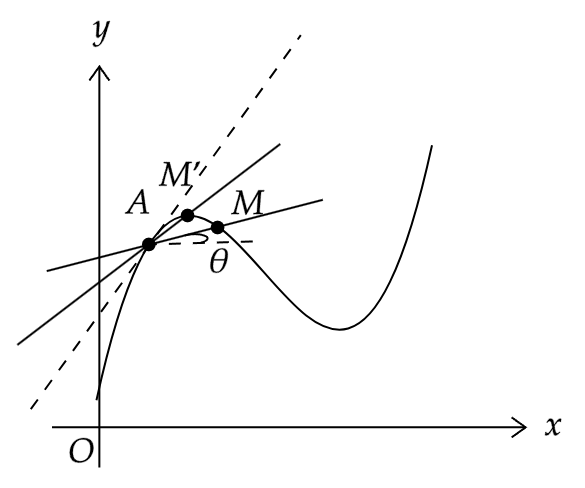
\includegraphics[width=0.6\textwidth]{Slides/figure/cattuyen.png}
        \caption{Cát tuyến của đồ thị hàm số}
    \end{figure}
    \end{column}
        \begin{column}{0.5\textwidth}
    Từ hình vẽ, ta thu được:
    \begin{equation}
    \tan\theta=\dfrac{f(x_M)-f(x_A)}{x_M-x_A}
    \end{equation}
    Khi lấy một điểm \(M'\) gần điểm \(A\) hơn \(M\) trên đồ thị, cát tuyến \(AM'\) sẽ gần với tiếp tuyến tại điểm \(A\) (đường nét đứt) hơn.
    \end{column}
    \end{columns}
\end{frame}
\begin{frame}{Đạo hàm}
    \begin{columns}
        \begin{column}{0.5\textwidth}
Khi điểm điểm \(M\) tiến gần đến điểm \(A\), độ dốc của cát tuyến \(AM\) sẽ tiến gần đến độ dốc của tiếp tuyến tại điểm \(A\):
\begin{figure}
    \centering
    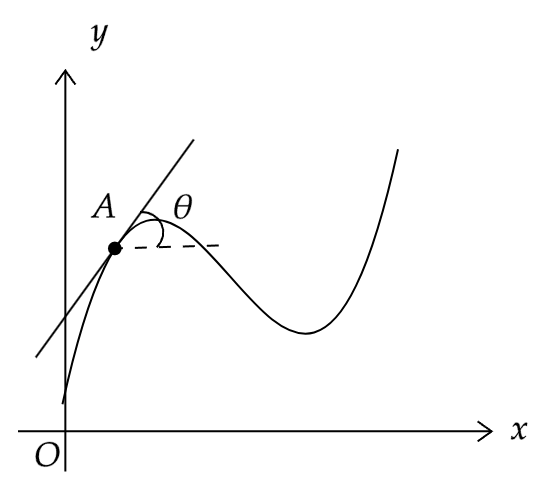
\includegraphics[width=0.6\textwidth]{Slides/figure/tieptuyen.png}
    \caption{Cát tuyến tiến gần đến tiếp tuyến}
\end{figure}
        \end{column}
        \begin{column}{0.5\textwidth}
Độ dốc của tiếp tuyến tại điểm \(A\) được tính bằng giới hạn:
\begin{equation}
    \tan\theta=\lim_{M\to A}\dfrac{f(x_M)-f(x_A)}{x_M-x_A}=f'(x_A)
\end{equation}
\(\longrightarrow\) Đạo hàm của hàm số tại điểm \(A\) phản ánh độ dốc của đồ thị tại điểm đó, cũng chính là tốc độ biến thiên của hàm số tại điểm đó.
        \end{column}
    \end{columns}
\end{frame}
\begin{frame}{Đạo hàm}
    Bảng đạo hàm của các hàm thông dụng:
    \begin{tcolorbox}[colback=blue!10, colframe=blue!50!black, title=]
    \begin{columns}
        \column{0.3\textwidth}
        \[
        \begin{aligned}
            &\dfrac{d}{dx}(x^n)=nx^{n-1}\\
            &\dfrac{d}{dx}(\sin x)=\cos x\\
            &\dfrac{d}{dx}(\tan x)=\sec^2 x
        \end{aligned}
        \]
    \column{0.3\textwidth}
    \[
    \begin{aligned}
        &\dfrac{d}{dx}a^x=a^x \ln a\\
        &\dfrac{d}{dx}(\cos x)=-\sin x\\
        &\dfrac{d}{dx}(\cot x)=-\csc^2 x
        \end{aligned}
    \]
    \end{columns}
    \end{tcolorbox}
    \end{frame}

    \begin{frame}{Đạo hàm}
\begin{columns}
    \begin{column}{0.5\textwidth}
\textbf{Ví dụ 1:} Một người di chuyển theo một đường thẳng. Kí hiệu \(x(t)\) là vị trí của người đó tại thời điểm \(t\).
\begin{figure}
    \centering
    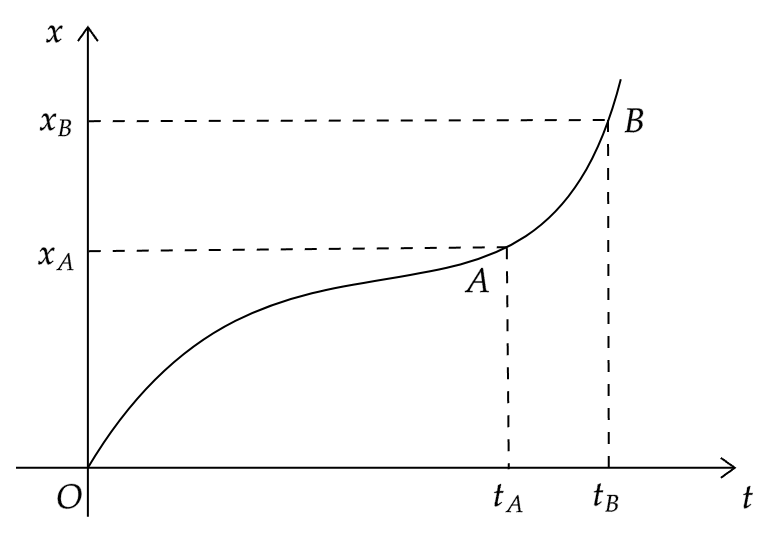
\includegraphics[width=0.9\textwidth]{Slides/figure/toc do trung binh.png}
\end{figure}
\end{column}
    \begin{column}{0.5\textwidth}
Tốc độ trung bình của người đó trong khoảng thời gian \([t_A, t_B]\) được tính bằng:
\begin{equation}
    \overline{v}_{AB}=\dfrac{x(t_B)-x(t_A)}{t_B-t_A}
\end{equation}
\end{column}
\end{columns}
\end{frame}

\begin{frame}{Đạo hàm}
\begin{columns}
    \begin{column}{0.5\textwidth}
Lấy một điểm \(B'\) gần điểm \(A\) hơn, ta thấy đồ thị hàm số \(x(t)\) gần giống đường thẳng \(AB'\) hơn:
\begin{figure}
    \centering
    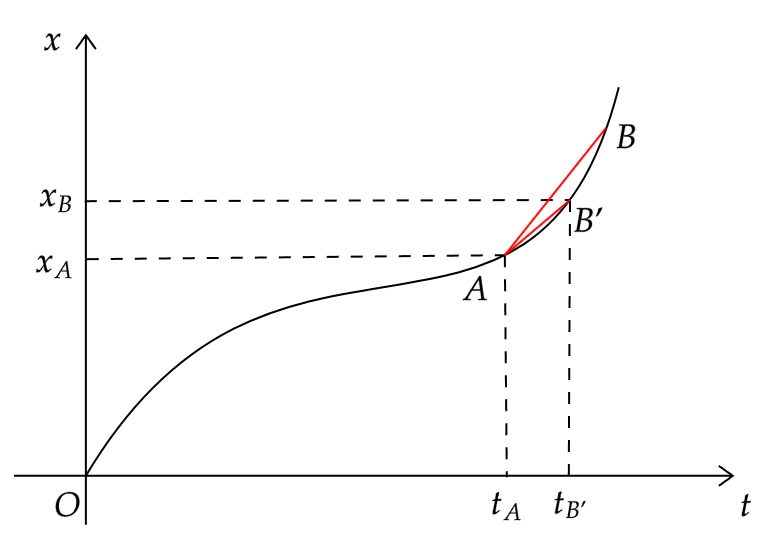
\includegraphics[width=0.9\textwidth]{Slides/figure/toc do tuc thoi.png}
\end{figure}
\end{column}
    \begin{column}{0.5\textwidth}
Như vậy, tốc độ trung bình trong khoảng thời gian \([t_A, t_B']\) sẽ gần với tốc độ tức thời tại thời điểm \(t_A\):
\begin{equation}
    v(t_A)=\lim_{B'\to A}\overline{v}_{AB'}
\end{equation}
Hay
\begin{equation}
    v(t_A)=\lim_{t_{B'} \to t_A}\dfrac{x(t_{B'})-x(t_A)}{t_{B'}-t_A}=x'(t_A)
\end{equation}
    \end{column}
\end{columns}
\end{frame}

\begin{frame}{Đạo hàm}
Ví dụ 2: Nước trong ấm siêu tốc có nhiệt độ \(T\), đang nhận công suất nhiệt \(\mathcal{P}_0\) từ ấm. Trong quá trình đó, nước đồng thời tỏa nhiệt ra môi trường (có nhiệt độ \(T_0\)) với công suất \(\mathcal{P}_1=k(T-T_0)\). Biết rằng nước có khối lượng \(m\) và nhiệt dung riêng là \(c\).
\begin{figure}
    \centering
    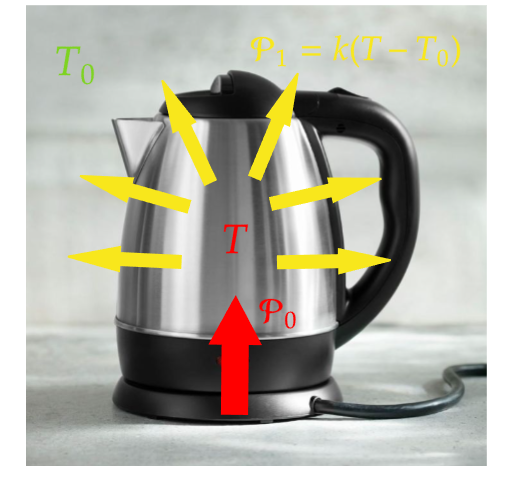
\includegraphics[width=0.25\textwidth]{Slides/figure/dunnuoc.png}
\end{figure}
Tính nhiệt độ của nước tại thời điểm \(t\), biết ban đầu nước có nhiệt độ \(T_0\).
\end{frame}
\begin{frame}{Đạo hàm}
\textbf{Giải:} Trong khoảng thời gian \(\Delta t\), nước nhận nhiệt lượng \(\Delta Q\) và tăng nhiệt độ một lượng \(\Delta T\).
\begin{columns}
    \begin{column}{0.5\textwidth}
\begin{equation}
\Delta Q=mc\Delta T
\end{equation}
\begin{equation}
\dfrac{\Delta Q}{\Delta t}=mc\dfrac{\Delta T}{\Delta t}
\end{equation}
\begin{equation}
\lim_{\Delta t\to 0}\dfrac{\Delta Q}{\Delta t}=mc\lim_{\Delta t\to 0}\dfrac{\Delta T}{\Delta t}
\end{equation}
\begin{equation}
    Q'(t)=mcT'(t)
\end{equation}
    \end{column}
    \begin{column}{0.5\textwidth}
    \end{column}
    \end{columns}
\end{frame}

\begin{frame}{Đạo hàm}
\textbf{Giải:} Trong khoảng thời gian \(\Delta t\), nước nhận nhiệt lượng \(\Delta Q\) và tăng nhiệt độ một lượng \(\Delta T\).
\begin{columns}
    \begin{column}{0.5\textwidth}
\begin{equation}
\Delta Q=mc\Delta T
\end{equation}
\begin{equation}
\dfrac{\Delta Q}{\Delta t}=mc\dfrac{\Delta T}{\Delta t}
\end{equation}
\begin{equation}
\lim_{\Delta t\to 0}\dfrac{\Delta Q}{\Delta t}=mc\lim_{\Delta t\to 0}\dfrac{\Delta T}{\Delta t}
\end{equation}
\begin{equation}
    Q'(t)=mcT'(t)
\end{equation}
    \end{column}
    \begin{column}{0.5\textwidth}
\begin{equation}
Q'(t)=\mathcal{P}_0-\mathcal{P}_1
\end{equation}
\begin{equation}
\boxed{mcT'(t)=\mathcal{P}_0-k(T-T_0)}
\end{equation}
\begin{equation}
    T(t)=T_0+\dfrac{\mathcal P_0}{k}(1-\exp(-kt/mc))
\end{equation}
    \end{column}
\end{columns}
\end{frame}

\begin{frame}{Tính toán số}
Giả sử ta muốn tính đạo hàm của \(y(x)\) bằng các công cụ lập trình, sẽ là tự nhiên nếu sử dụng trục tiếp định nghĩa của đạo hàm:
\[y(x_0+\epsilon)\approx y(x_0)+\epsilon y'(x_0).\] Ở đây \(\epsilon\) là một con số rất nhỏ, ví dụ như \(0.01\), hay nếu cần chính xác hơn, có thể là \(0.001\),v.v. Như vậy, việc ta cần làm chỉ là khai báo hàm \(y(x)\) rồi chọn một bước nhảy thích hợp. 
\end{frame}

